% !Mode:: "TeX:UTF-8"%確保文檔utf-8編碼
\documentclass[tikz,border=2pt]{standalone}
\usepackage{pgfplots}
\pgfplotsset{compat=newest}
\usetikzlibrary{backgrounds,calc}

\begin{document}
\usetikzlibrary{backgrounds,calc}
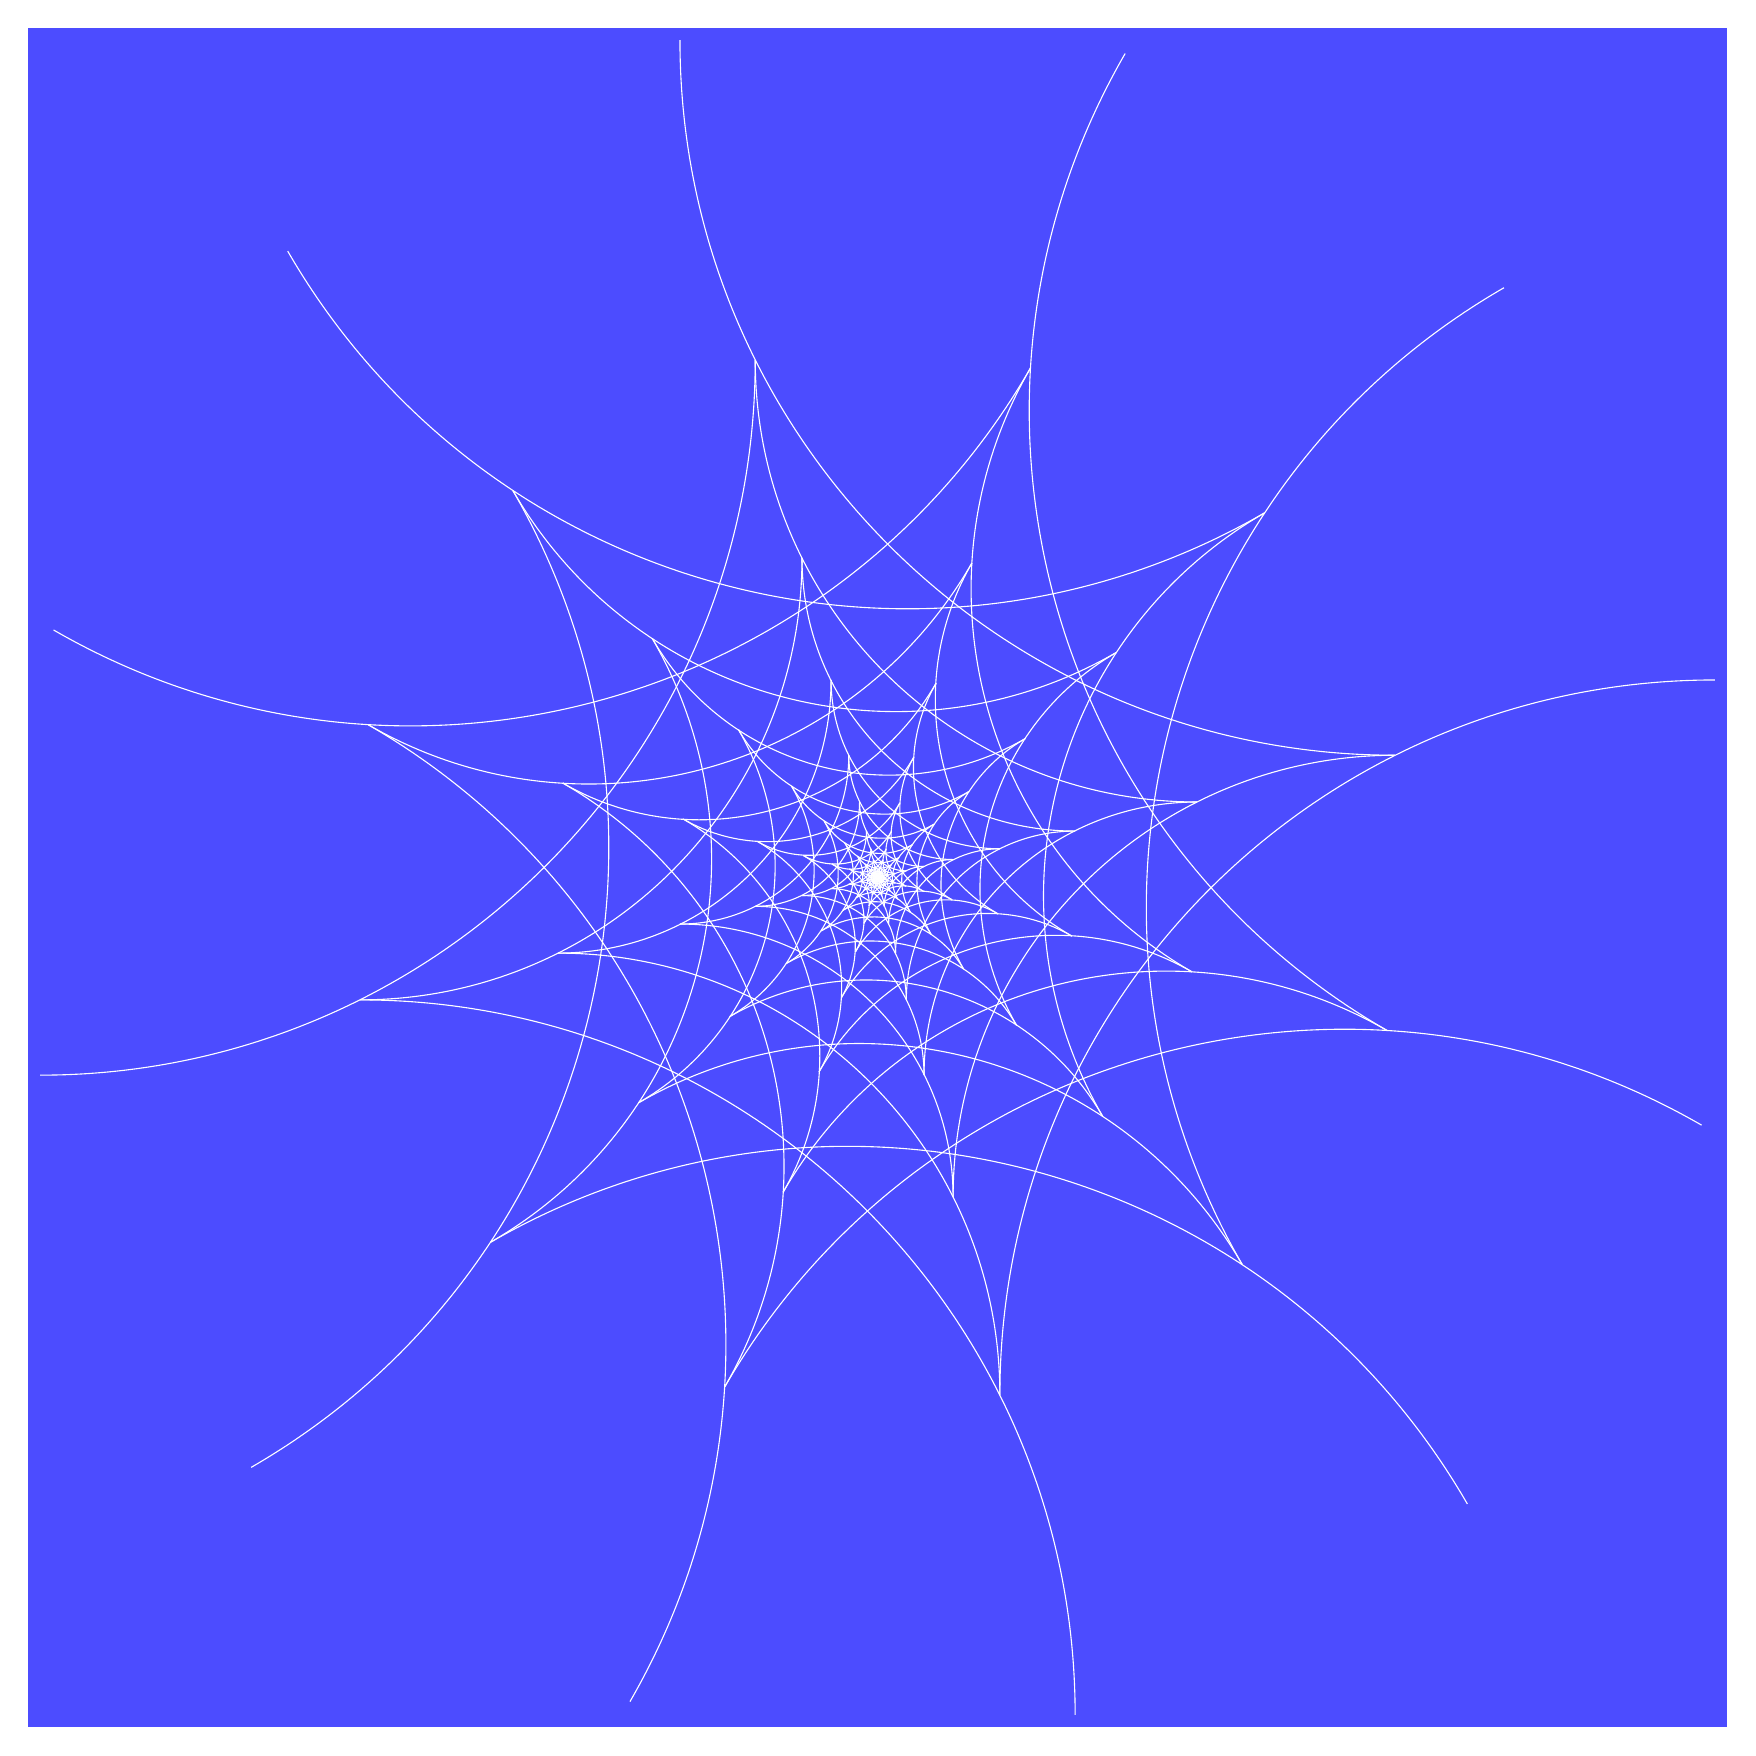
\begin{tikzpicture}[background rectangle/.style={fill=blue!70},show background rectangle]
  % Create some counters for holding the Fibonacci numbers
  \newcounter{a}
  \newcounter{b}
  \newcounter{temp}

\def\n{12}
\foreach \i in {1,...,\n}
{
\begin{scope}[rotate=\i*360/\n]
% Initialize the counters
  \setcounter{a}{0}
  \setcounter{b}{1}

  % The spiral will start at the origin
  \coordinate (0) at (0,0);

  % This loop defines the number of turns in the spiral. Note that we
  % will have to be careful not to overflow our counters or make the
  % spiral too large for TeX to handle. This is easy to do as the
  % Fibonacci sequence grows exponentially.
  \foreach \i in {1,...,18}
  {
    % Get the "name" of the last point on the spiral
    \pgfmathsetmacro{\lastpoint}{\i-1}

    % Compute the angle for this turn of the spiral
    \pgfmathsetmacro{\startangle}{mod(\i-1,4) * 90}

    % Draw this turn of the spiral and remember the point where we end 
    \draw[color=white] (\lastpoint) arc 
      (\startangle  : \startangle - 90 : \value{b}/10.0pt) coordinate (\i);
   % Compute the next Fibonacci number
    \setcounter{temp}{\value{b}}
    \addtocounter{b}{\value{a}}
    \setcounter{a}{\value{temp}}
 }

\end{scope}
}



\end{tikzpicture}
\end{document}